

\section{Komplexe Zahlen}

\begin{lemma}{Fundamentalsatz der Algebra}\\
Eine algebraische Gleichung n-ten Grades mit komplexen Koeffizienten:
$$a_nz^n + a_{n-1}z^{n-1} + \cdots + a_1z + a_0 = 0$$
besitzt in $\mathbb{C}$ genau n Lösungen (mit Vielfachheiten gezählt).
\end{lemma}

\begin{concept}{Komplexe Zahlen}\\
Die Menge der komplexen Zahlen $\mathbb{C}$ erweitert die reellen Zahlen $\mathbb{R}$ durch Einführung der imaginären Einheit $i$ mit der Eigenschaft:
$$i^2 = -1$$

Eine komplexe Zahl $z$ ist ein geordnetes Paar $(x,y)$ mit $x,y \in \mathbb{R}$:
$$z = x + iy$$

Die Menge aller komplexen Zahlen ist definiert als:
$$\mathbb{C} = \{z \mid z = x + iy \text{ mit } x,y \in \mathbb{R}\}$$
\end{concept}



\begin{definition}{Bestandteile komplexer Zahlen}\\
\begin{minipage}[t]{0.6\textwidth}
    \vspace{-7mm}
    \textbf{Realteil:} $\operatorname{Re}(z) = x$\\
    \textbf{Imaginärteil:} $\operatorname{Im}(z) = y$\\
    \textbf{Betrag:} $|z| = \sqrt{x^2 + y^2} = \sqrt{z \cdot z^*}$\\
    \textbf{Konjugation:} $\overline{z} = x - iy$
\end{minipage}
\begin{minipage}{0.35\textwidth}
    \vspace{-3mm}
    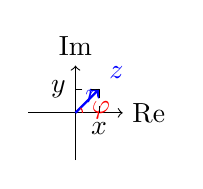
\begin{tikzpicture}[scale=0.3]
        % Coordinate axes
        \draw[->] (-2,0) -- (2,0) node[right] {Re};
        \draw[->] (0,-2) -- (0,2) node[above] {Im};
        
        % Example point and vector
        \draw[thick,blue,->] (0,0) -- (1,1) node[above right] {$z$};
        
        % Angle and labels
        \draw[red] (0.3,0) arc (0:45:0.3) node[midway,right] {$\varphi$};
        
        % Components
        \draw[dashed] (1,1) -- (1,0) node[below] {$x$};
        \draw[dashed] (1,1) -- (0,1) node[left] {$y$};
        
        % Radius
        \node[blue] at (0.7,0.7) {$r$};
    \end{tikzpicture}
\end{minipage}
\end{definition}


\begin{concept}{Darstellungsformen}
\begin{itemize}
    \item Normalform: $z = x + iy$
    \item Trigonometrische Form: $z = r(\cos\varphi + i\sin\varphi)$
    \item Exponentialform: $z = re^{i\varphi}$
\end{itemize}
\end{concept}

\begin{KR}{Umrechnung zwischen Darstellungsformen komplexer Zahlen}
\paragraph{Von Normalform in trigonometrische Form/Exponentialform}
\begin{enumerate}
   \item Berechne Betrag $r = \sqrt{x^2 + y^2}$
   \item Berechne Winkel mit einer der Formeln: 
   \begin{itemize}
       \item $\varphi = \arctan(\frac{y}{x})$ falls $x > 0$
       \item $\varphi = \arctan(\frac{y}{x}) + \pi$ falls $x < 0$
       \item $\varphi = \frac{\pi}{2}$ falls $x = 0, y > 0$
       \item $\varphi = -\frac{\pi}{2}$ falls $x = 0, y < 0$
       \item $\varphi$ unbestimmt falls $x = y = 0$
   \end{itemize}
   \item Trigonometrische Form: $z = r(\cos\varphi + i\sin\varphi)$
   \item Exponentialform: $z = re^{i\varphi}$
\end{enumerate}

\paragraph{Von trigonometrischer Form in Normalform}
\begin{enumerate}
   \item Realteil: $x = r\cos\varphi$
   \item Imaginärteil: $y = r\sin\varphi$
   \item Normalform: $z = x + iy$
\end{enumerate}

\paragraph{Von Exponentialform in Normalform/trigonometrische Form}
\begin{enumerate}
   \item Trigonometrische Form durch Euler-Formel:\\
   $re^{i\varphi} = r(\cos\varphi + i\sin\varphi)$
   \item Dann wie oben in Normalform umrechnen
\end{enumerate}

\paragraph{Wichtige Hinweise:}
\begin{itemize}
   \item Achten Sie auf das korrekte Quadranten beim Winkel
   \item Winkelfunktionen im Bogenmaß verwenden
   \item Bei Umrechnung in Normalform Euler-Formel nutzen
   \item Vorzeichen bei Exponentialform beachten
\end{itemize}
\end{KR}




\begin{theorem}{Rechenoperationen mit komplexen Zahlen}\\
Für $z_1 = x_1 + iy_1$ und $z_2 = x_2 + iy_2$ gilt:
\vspace{1mm}\\
\begin{minipage}[t]{0.45\textwidth}
    \textbf{Addition:}\\
    $z_1 + z_2 = (x_1 + x_2) + i(y_1 + y_2)$
\end{minipage}
\hspace{3mm}
\begin{minipage}[t]{0.45\textwidth}
    \textbf{Subtraktion:}\\
    $z_1 - z_2 = (x_1 - x_2) + i(y_1 - y_2)$
\end{minipage}

\begin{minipage}{0.28\textwidth}
    \textbf{Multiplikation:}
\end{minipage}
\begin{minipage}{0.68\textwidth}
    \begin{align*}
        z_1 \cdot z_2 &= (x_1x_2 - y_1y_2) + i(x_1y_2 + x_2y_1)\\
        &= r_1r_2e^{i(\varphi_1 + \varphi_2)} \text{ (in Exponentialform)}
    \end{align*}
\end{minipage}



\textbf{Division:}
\begin{align*}
    \frac{z_1}{z_2} &= \frac{z_1 \cdot z_2^*}{z_2 \cdot z_2^*} = \frac{(x_1x_2 + y_1y_2) + i(y_1x_2 - x_1y_2)}{x_2^2 + y_2^2}\\
    &= \frac{r_1}{r_2}e^{i(\varphi_1 - \varphi_2)} \text{ (in Exponentialform)}
\end{align*}
\end{theorem}

\begin{corollary}{Potenzen und Wurzeln}\\
Für eine komplexe Zahl in Exponentialform $z = re^{i\varphi}$ gilt:
\begin{itemize}
    \item n-te Potenz: $z^n = r^ne^{in\varphi} = r^n(\cos(n\varphi) + i\sin(n\varphi))$
    \item n-te Wurzel: $z_k = \sqrt[n]{r}e^{i\frac{\varphi + 2\pi k}{n}}$, $k = 0,1,\ldots,n-1$
\end{itemize}
\end{corollary}

\begin{example2}{Komplexe Operationen}
Gegeben $z_1 = 1+i$ und $z_2 = 2-i$:

\paragraph{Umrechnung in Polarform:}
\begin{itemize}
    \item $z_1: r_1 = \sqrt{2}$, $\varphi_1 = \frac{\pi}{4}$
    \item $z_2: r_2 = \sqrt{5}$, $\varphi_2 = -\arctan(\frac{1}{2})$
\end{itemize}

\paragraph{Berechnungen:}
\begin{itemize}
    \item $z_1 \cdot z_2 = (2-i)(1+i) = (2+1) + i(2-1) = 3+i$
    \item $z_1^3 = (\sqrt{2})^3(\cos(\frac{3\pi}{4}) + i\sin(\frac{3\pi}{4}))$
\end{itemize}
\end{example2}

\raggedcolumns
\columnbreak

\section{Eigenwerte und Eigenvektoren}

\begin{definition}{Eigenwerte und Eigenvektoren}\\
Für eine Matrix $A \in \mathbb{R}^{n\times n}$ heißt $\lambda \in \mathbb{C}$ Eigenwert von $A$, wenn es einen Vektor $x \in \mathbb{C}^n \backslash \{0\}$ gibt mit:
\vspace{-2mm}\\
$$Ax = \lambda x$$
Der Vektor $x$ heißt dann Eigenvektor zum Eigenwert $\lambda$.
\end{definition}

\begin{concept}{Bestimmung von Eigenwerten}\\
Ein Skalar $\lambda$ ist genau dann Eigenwert von $A$, wenn gilt:
\vspace{-2mm}\\
$$\det(A - \lambda I_n) = 0 \text{(charakteristische Gleichung)}$$
$$\text{charakteristisches Polynom von }A : p(\lambda) = \det(A - \lambda I_n)$$
\end{concept}

\begin{theorem}{Eigenschaften von Eigenwerten}
Für eine Matrix $A \in \mathbb{R}^{n\times n}$ gilt:

\begin{minipage}{0.5\textwidth}
    $$\text{Determinante: } \det(A) = \prod_{i=1}^n \lambda_i $$
\end{minipage}
\begin{minipage}{0.5\textwidth}
    $$\text{Spur: }\operatorname{tr}(A) = \sum_{i=1}^n \lambda_i$$
\end{minipage}

\begin{itemize}
    \item Bei Dreiecksmatrix sind die Diagonalelemente die Eigenwerte
    \item Ist $\lambda$ Eigenwert von $A$, so ist $\frac{1}{\lambda}$ Eigenwert von $A^{-1}$
\end{itemize}
\end{theorem}

\begin{formula}{Vielfachheiten}
Für einen Eigenwert $\lambda$ unterscheidet man:
\begin{itemize}
    \item Algebraische Vielfachheit: \\Vielfachheit als Nullstelle des charakteristischen Polynoms
    \item Geometrische Vielfachheit: \\Dimension des Eigenraums $= n - \operatorname{rg}(A-\lambda I_n)$
\end{itemize}
Die geometrische Vielfachheit ist stets kleiner oder gleich der algebraischen Vielfachheit.
\end{formula}

\begin{definition}{Diagonalisierbarkeit}
Eine Matrix $A$ ist genau dann diagonalisierbar, wenn sie $n$ linear unabhängige Eigenvektoren besitzt. Dies ist äquivalent zu:
\begin{itemize}
    \item Die algebraischen Vielfachheiten der Eigenwerte entsprechen den geometrischen Vielfachheiten
    \item Die Summe der geometrischen Vielfachheiten ist $n$
    \item Die Matrix $A$ ist ähnlich zu einer Diagonalmatrix
    \item Die Matrix $A$ hat $n$ linear unabhängige Eigenvektoren
\end{itemize}
\end{definition}

\begin{concept}{Ähnliche Matrizen}\\
Zwei Matrizen $A,B \in \mathbb{R}^{n\times n}$ heißen ähnlich, wenn es eine reguläre Matrix $T$ gibt mit:
$$B = T^{-1}AT$$

Eine Matrix $A$ heißt diagonalisierbar, wenn sie ähnlich zu einer Diagonalmatrix $D$ ist:
$$D = T^{-1}AT$$
\end{concept}

\begin{theorem}{Eigenschaften ähnlicher Matrizen}\\
Für ähnliche Matrizen $A$ und $B = T^{-1}AT$ gilt:
\begin{enumerate}
    \item $A$ und $B$ haben dieselben Eigenwerte mit gleichen algebraischen Vielfachheiten
    \item Ist $x$ Eigenvektor von $B$ zum Eigenwert $\lambda$, so ist $Tx$ Eigenvektor von $A$ zum Eigenwert $\lambda$
    \item Bei Diagonalisierbarkeit:
    \begin{itemize}
        \item Die Diagonalelemente von $D$ sind die Eigenwerte von $A$
        \item Die Spalten von $T$ sind die Eigenvektoren von $A$
    \end{itemize}
\end{enumerate}
\end{theorem}

\begin{KR}{Bestimmung von Eigenwerten}

\paragraph{Charakteristisches Polynom aufstellen}
\begin{itemize}
    \item $p(\lambda) = \det(A-\lambda I)$ berechnen und auf Standardform bringen
    \item  Spezialfälle:
    \begin{itemize}
        \item Bei $2 \times 2$ Matrizen direkt: $\det(A - \lambda I)$
        \item Bei $3 \times 3$ Matrizen: Entwicklung nach einer Zeile/Spalte
        \item Bei größeren Matrizen: Spezielle Eigenschaften nutzen
              (z.B. Dreiecksform, Symmetrie)
    \end{itemize}
\end{itemize}
    
    \paragraph{Polynom vereinfachen und auf Nullform bringen}
    \begin{itemize}
        \item Ausmultiplizieren
        \item Zusammenfassen nach Potenzen von $\lambda$
        \item Form: $p(\lambda) = (-1)^n\lambda^n + a_{n-1}\lambda^{n-1} + \cdots + a_1\lambda + a_0$
    \end{itemize}

    \paragraph{Nullstellen bestimmen}
    \begin{itemize}
        \item Quadratische Formel für $n=2$ (Grad des Polynoms)
        \item Cardano-Formel oder Substitution für $n=3$
        \item Numerische Verfahren für $n>3$
    \end{itemize}

    \paragraph{Vielfachheiten bestimmen}
    \begin{itemize}
        \item Algebraische Vielfachheit: Nullstellenordnung
        \item Geometrische Vielfachheit: $n-\operatorname{rang}(A-\lambda I)$
    \end{itemize}
\end{KR}

\begin{example2}{Charakteristisches Polynom}\\
Bestimmen Sie die Eigenwerte von:
$A = \begin{psmallmatrix}
2 & -1 & 0 \\
-1 & 2 & -1 \\
0 & -1 & 2
\end{psmallmatrix}$

\paragraph{Lösung:}
\begin{enumerate}
    \item $p(\lambda) = \det(A-\lambda I)$:
    $\begin{vsmallmatrix}
    2-\lambda & -1 & 0 \\
    -1 & 2-\lambda & -1 \\
    0 & -1 & 2-\lambda
    \end{vsmallmatrix}$
    \vspace{1mm}\\
    \item Determinante:
    $p(\lambda) = (2-\lambda)^3 - 2(2-\lambda) = -\lambda^3 + 6\lambda^2 - 11\lambda + 6$
    \vspace{1mm}\\
    \item Nullstellen:
    $\lambda_1 = 1, \lambda_2 = 2, \lambda_3 = 3$
\end{enumerate}
\end{example2}

\begin{KR}{Bestimmung von Eigenvektoren}

\paragraph{Eigenvektoren bestimmen}
\begin{enumerate}
    \item Für jeden Eigenwert $\lambda_i$:
    \begin{itemize}
        \item Matrix $(A - \lambda_i I)$ aufstellen
        \item Homogenes LGS $(A - \lambda_i I)x = 0$ lösen
        \item Lösungsvektor normieren falls gewünscht
    \end{itemize}

    \item Bei mehrfachen Eigenwerten:
    \begin{itemize}
        \item Geometrische Vielfachheit bestimmen
        \item Basis des Eigenraums bestimmen
        \item Linear unabhängige Eigenvektoren finden
    \end{itemize}
\end{enumerate}

\paragraph{Kontrolle}
\begin{itemize}
    \item Für jeden Eigenvektor $x_i$ prüfen: $Ax_i = \lambda_i x_i$
    \item Bei symmetrischen Matrizen: Orthogonalität der Eigenvektoren prüfen
    \item Linear unabhängigkeit der Eigenvektoren überprüfen
    \item Bei $2 \times 2$ Matrix: $\lambda_1 + \lambda_2 = \operatorname{tr}(A)$ und $\lambda_1 \cdot \lambda_2 = \det(A)$
    \item Bei $3 \times 3$ Matrix zusätzlich: $\sum \lambda_i = \operatorname{tr}(A)$ und $\prod \lambda_i = \det(A)$
    \item Bei reellen Matrizen: Komplexe Eigenwerte treten in konjugierten Paaren auf
\end{itemize}

\paragraph{Spezialfälle beachten}
\begin{itemize}
    \item Bei Dreiecksmatrizen: Eigenwerte sind die Diagonalelemente
    \item Bei symmetrischen Matrizen: Alle Eigenwerte sind reell
    \item Bei orthogonalen Matrizen: $|\lambda_i| = 1$ für alle Eigenwerte
    \item Bei nilpotenten Matrizen: Alle Eigenwerte sind 0\\
    nilpotente Matrix: $A^k = 0$ für ein $k \in \mathbb{N}$
\end{itemize}
\end{KR}

\begin{example2}{Eigenwertberechnung}
Gegeben ist die Matrix
$A = \begin{psmallmatrix} 
2 & 1 & 0 \\
1 & 2 & 1 \\
0 & 1 & 2
\end{psmallmatrix}$

1. Charakteristisches Polynom aufstellen:
   $$\det(A - \lambda I) = \begin{vsmallmatrix} 
   2-\lambda & 1 & 0 \\
   1 & 2-\lambda & 1 \\
   0 & 1 & 2-\lambda
   \end{vsmallmatrix}$$
   
2. Entwicklung nach 1. Zeile:
   $$p(\lambda) = (2-\lambda)\begin{vsmallmatrix}
   2-\lambda & 1 \\
   1 & 2-\lambda
   \end{vsmallmatrix} - 1\begin{vsmallmatrix}
   1 & 1 \\
   1 & 2-\lambda
   \end{vsmallmatrix}$$
   
3. Ausrechnen:
   $$p(\lambda) = (2-\lambda)((2-\lambda)^2 - 1) - ((2-\lambda) - 1)
   = -\lambda^3 + 6\lambda^2 - 11\lambda + 6$$
   
4. Nullstellen bestimmen:
   $\lambda_1 = 1, \lambda_2 = 2, \lambda_3 = 3$
\vspace{1mm}\\
5. Eigenvektoren bestimmen für $\lambda_1 = 1$:
   $$(A - I)x = 0 \text{ führt zu } x_1 = \begin{psmallmatrix} 1 \\ -2 \\ 1 \end{psmallmatrix}$$
\end{example2}

\begin{example2}{Eigenvektoren}
Bestimmen Sie die Eigenvektoren zum Eigenwert $\lambda=2$ der Matrix:
$$A = \begin{psmallmatrix}
2 & 1 & 0 \\
0 & 2 & 0 \\
0 & -1 & 2
\end{psmallmatrix}$$

\paragraph{Lösung:}
\begin{enumerate}
    \item $(A-2I)x = 0$:
    $$\begin{psmallmatrix}
    0 & 1 & 0 \\
    0 & 0 & 0 \\
    0 & -1 & 0
    \end{psmallmatrix} \begin{psmallmatrix}
    x_1 \\ x_2 \\ x_3
    \end{psmallmatrix} = \begin{psmallmatrix}
    0 \\ 0 \\ 0
    \end{psmallmatrix}$$
    
    \item Homogenes System lösen:
    \begin{itemize}
        \item $x_2 = 0$ (aus 1. Zeile)
        \item $x_1, x_3$ frei wählbar
    \end{itemize}
    
    \item Basis des Eigenraums:
    $$v_1 = \begin{psmallmatrix} 1 \\ 0 \\ 0 \end{psmallmatrix}, 
    v_2 = \begin{psmallmatrix} 0 \\ 0 \\ 1 \end{psmallmatrix}$$
\end{enumerate}
\end{example2}



\begin{example2}{Eigenwerte und Eigenvektoren}
Bestimmen Sie Eigenwerte und -vektoren von:
$$A = \begin{psmallmatrix}
2 & -1 \\
-1 & 2
\end{psmallmatrix}$$

\paragraph{Lösung:}
\begin{enumerate}
    \item Charakteristisches Polynom:
    $$\det(A-\lambda I) = \begin{vmatrix} 
    2-\lambda & -1 \\
    -1 & 2-\lambda
    \end{vmatrix} = (2-\lambda)^2 - 1 = 0$$
    
    \item Eigenwerte: $\lambda_1 = 3$, $\lambda_2 = 1$
    
    \item Eigenvektoren für $\lambda_1 = 3$:
    $$(A-3I)x = \begin{psmallmatrix}
    -1 & -1 \\
    -1 & -1
    \end{psmallmatrix}x = 0 \Rightarrow x_1 = \begin{psmallmatrix}
    1 \\
    1
    \end{psmallmatrix}$$
    
    \item Eigenvektoren für $\lambda_2 = 1$:
    $$(A-I)x = \begin{psmallmatrix}
    1 & -1 \\
    -1 & 1
    \end{psmallmatrix}x = 0 \Rightarrow x_2 = \begin{psmallmatrix}
    1 \\
    -1
    \end{psmallmatrix}$$
\end{enumerate}
\end{example2}






